\documentclass{ocbeameruni}


\setdefaultlanguage[babelshorthands=true]{german}


% Nur benötigt für die Beispiel-Listings!
\usepackage{listings}
\lstloadlanguages{[LaTeX]TeX}
\lstset{%
  basicstyle=\small \ttfamily,
  breaklines=true,
}

\newcommand{\R}{\mathbb{R}}


\title{Organic Computing 2}
\subtitle{Lösungsvorschlag Blatt03}
\date{\today}
\author{Lukas Huhn \and Qiang Chang \and Victor Gerling \and Daniel Bossert}
\institute{%
  Universität Augsburg\\
  Institut für Informatik\\
  Lehrstuhl für Organic Computing
}


\begin{document}


\maketitle


\begin{frame}{Gliederung}
  \setbeamertemplate{section in toc}[sections numbered]
  \tableofcontents
\end{frame}


\section{Aufgabe 01}

\begin{frame}{Attribut City}
    \begin{itemize}
    \item Beispiele: 0, 1, 2(Cities sind mit 0 bis n durchnummeriert)
    \item n
    \end{itemize}
\end{frame}

\begin{frame}{Attribut Route}
    \begin{itemize}
    \item Beispiele: [(0,1),(1,2),(1,3)], [(0,2), (2,1), (1,3)], [(0,3), (3,1), (1,2)]
    \item n!
    \end{itemize}
\end{frame}

\begin{frame}{Attribut Pheromone}
    \begin{itemize}
    \item Beispiele: 0.000002, 0.0002, 0.0000001
    \item Kontinierlicher Wertebereich, unendlich
    \end{itemize}
\end{frame}

\begin{frame}{1.3 Len}
    \begin{center}
    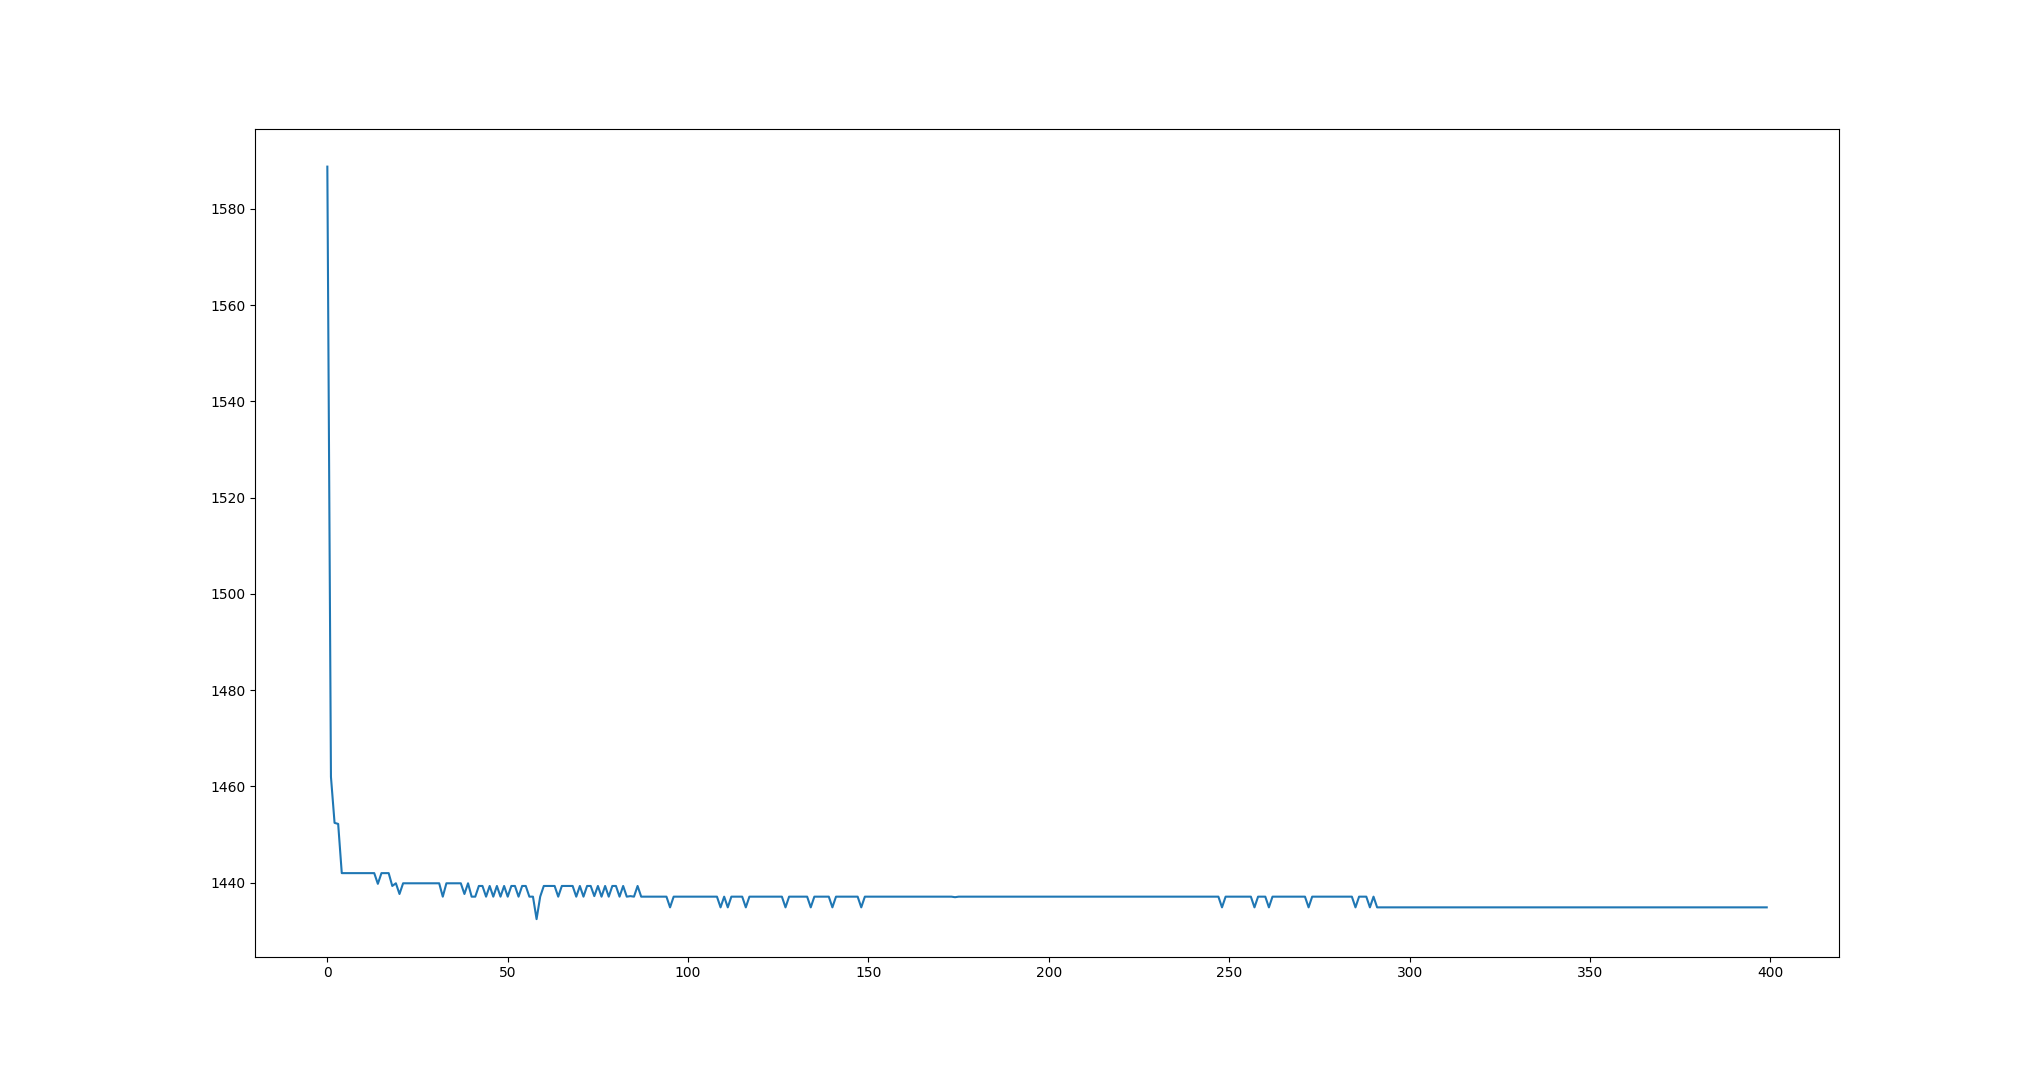
\includegraphics[scale=0.2]{Avg_len_per_iter.png}
    \end{center}
\end{frame}

\begin{frame}{1.3 Emerg}
    \begin{center}
    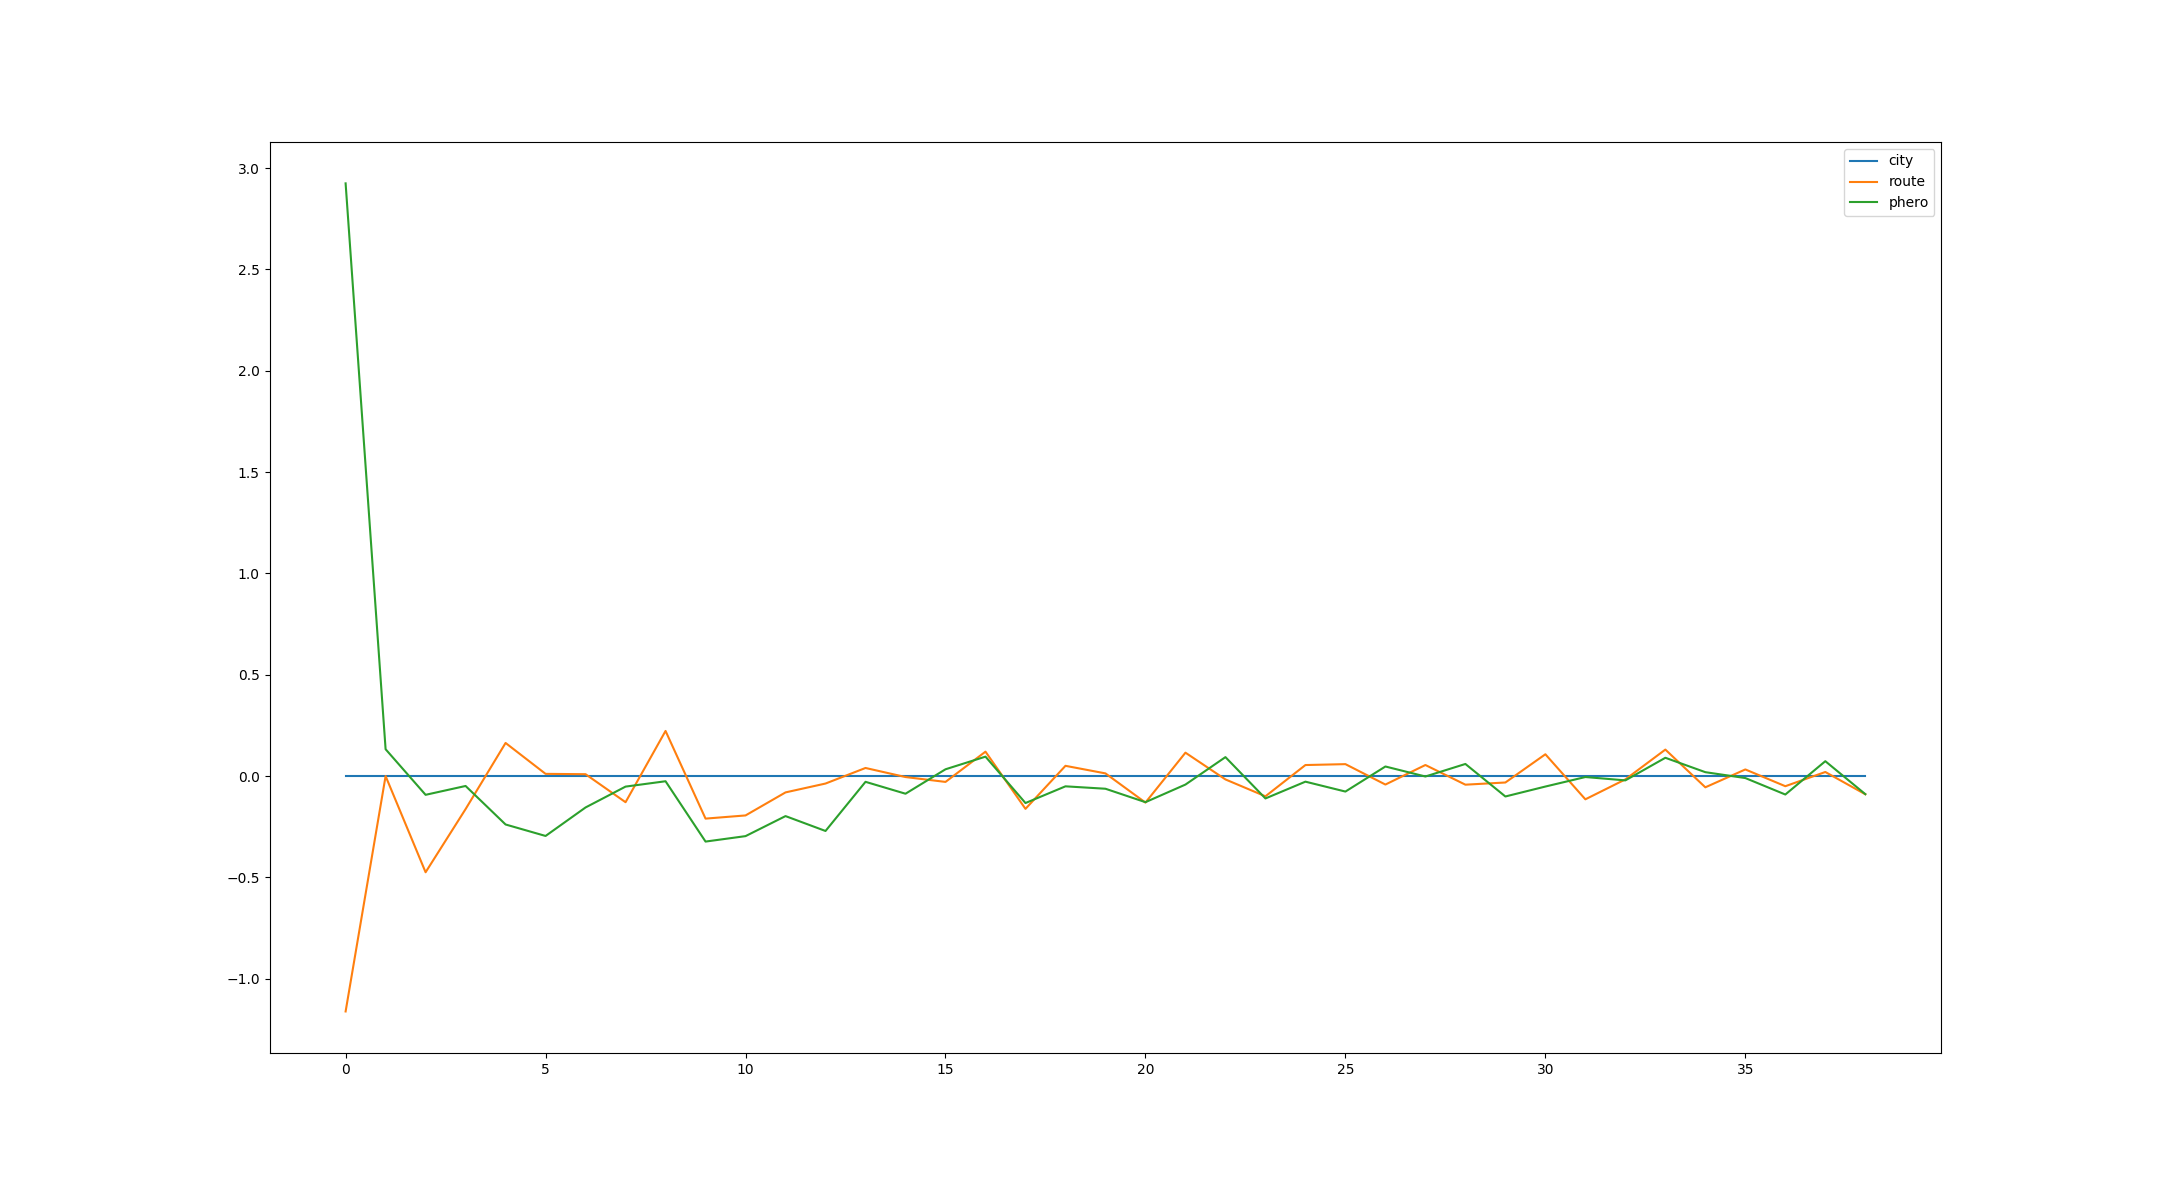
\includegraphics[scale=0.2]{Emerg_per_iter.png}
    \end{center}
\end{frame}

\begin{frame}{1.3 Spider}
    \begin{center}
    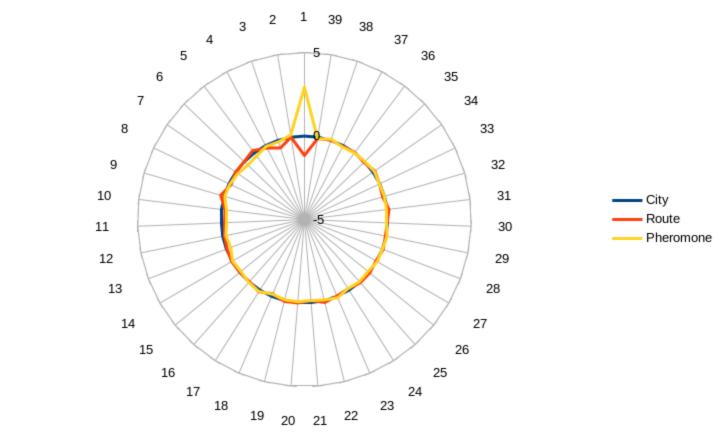
\includegraphics[scale=0.5]{spider_emerg.png}
    \end{center}
\end{frame}

\section{Aufgabe 4}

\begin{frame}{Aufgabe 4}
    \begin{itemize}
    \item Intel® Core™ i5-5257U CPU @ 2.70GHz × 4, 8GB Ram
    \item n=10: ~1.82 seconds, ants=10, iter=400 $\Rightarrow$ Routes=4000
    \item n=20: ~6.6 seconds, ants=15, iter=400 $\Rightarrow$ Routes=6000
    \item n=30: ~20 seconds, ants=20, iter=500 $\Rightarrow$ Routes=10000
    \end{itemize}
\end{frame}

\end{document}
% Local Variables:
% TeX-engine: xetex
% End:
